\documentclass{article}
\usepackage{fullpage}

%load needed packages
\usepackage{graphicx}
\usepackage{array}
\usepackage{booktabs}
\usepackage[utf8]{inputenc}
\usepackage[T1]{fontenc}
\usepackage{hyperref}


\usepackage{float}  % Necesario para [H]
\usepackage{listings}
\usepackage{xcolor}

\definecolor{codegreen}{HTML}{5AB2FF}
\definecolor{morado}{HTML}{AD88C6}
\definecolor{BG}{HTML}{EEEEEE}
\definecolor{azul}{HTML}{4D869C}
\definecolor{sqlblue}{HTML}{FF8C00} % Color para las palabras clave SQL
\usepackage{listings}
\usepackage{xcolor}


%estilo python
\usepackage{xcolor}

\usepackage{amsmath}
\usepackage{amssymb}
\usepackage{booktabs} % Para las tablas bonitas como \toprule, \midrule, etc.

% Define the colors for the style
\definecolor{BG}{rgb}{0.95,0.95,0.95}  % Background color
\definecolor{keywordcolor}{rgb}{0.0,0.0,1.0} % Blue for keywords
\definecolor{commentcolor}{rgb}{0.0,0.5,0.0} % Green for comments
\definecolor{stringcolor}{rgb}{1.0,0.0,0.0}  % Red for strings
\definecolor{attributecolor}{rgb}{0.8,0.3,0.8} % Purple for attributes
\definecolor{importcolor}{rgb}{0.0,0.6,0.6} % Teal for import statements

% Define the style for Python code
\lstdefinestyle{mypython}{
	backgroundcolor=\color{BG},   % Background color
	basicstyle=\footnotesize\ttfamily,  
	breaklines=true,                  
	language=Python,                  
	keywordstyle=\color{keywordcolor},    
	commentstyle=\color{commentcolor}, 
	stringstyle=\color{stringcolor},
	frame=shadowbox, 
	morekeywords={model},  % Add 'model' to keywords
	keywordstyle=[2]\color{importcolor}, % Color for import statements
	sensitive=true,       % Case sensitive
	morecomment=[s]{"""}{"} % Allows for multi-line strings
}



\lstset{style=mypython}
% Estilo para DDL
\lstdefinestyle{ddlstyle}{
	language=SQL,
	backgroundcolor=\color{BG},
	commentstyle=\color{codegreen},
	basicstyle=\ttfamily\small,
	keywordstyle=\color{azul},
	stringstyle=\color{morado},
	showstringspaces=false,
	breaklines=true,
	frame=shadowbox,
	numbers=left,
	numberstyle=\tiny\color{gray},
	captionpos=b,
}

% Estilo para SQL
\lstdefinestyle{sqlstyle}{
	language=SQL,
	backgroundcolor=\color{BG},
	commentstyle=\color{codegreen},
	basicstyle=\ttfamily\small,
	keywordstyle=\color{sqlblue}, % Color diferente para palabras clave SQL
	stringstyle=\color{morado},
	showstringspaces=false,
	breaklines=true,
	frame=shadowbox,
	numbers=left,
	numberstyle=\tiny\color{gray},
	captionpos=b,
}

\begin{document}



% Portada
\begin{titlepage}
	\centering
	\vspace*{3cm}
	
	% Título destacado
	{\Huge \textbf{Lab 3: Drug-Protein Binding Affinity Prediction}\\[0.5cm]}
	
	% Espacio y logotipo (si lo tienes, por ejemplo el logo de tu universidad)
	\vspace{2cm}
	
\includegraphics[width=0.3\textwidth]{images/uma_logo.jpg}\\[1cm]
	
	% Nombre del autor
	{\LARGE \textbf{Alejandro Silva Rodríguez}\\[0.5cm]}
	{\LARGE \textbf{Marta Cuevas Rodríguez}\\[0.5cm]}
	{\large \textit{Aprendizaje Computacional}\\
		Universidad de Málaga\\
		}
	
	\vfill
	
	% Fecha en la parte inferior de la página
	{\large Diciembre 2024}
\end{titlepage}

% indice
\tableofcontents

\newpage

\begin{abstract}
	This report presents the results of reproducing the work described in the paper "TEFDTA: A Transformer Encoder and Fingerprint Representation Combined Prediction Method for Bonded and Non-Bonded Drug–Target Affinities" by Zongquan Li et al \cite{lizongquan2024tefdta}. We faithfully implemented the methods and experiments detailed in the paper, using the publicly available datasets and code. Our findings demonstrate consistent results with those reported in the original work, confirming the validity and reproducibility of the TEFDTA model. 
\end{abstract}

\section{Introduction}
The prediction of drug–target interactions (DTI) is a critical challenge in drug discovery, as it determines the binding affinity between small molecules and specific proteins. Recent advancements in deep learning have significantly improved prediction accuracy, yet many methods struggle with covalent interactions, which are increasingly relevant in therapeutic research.
\\

The TEFDTA model introduced by Zongquan Li et al. combines transformer encoders with fingerprint-based molecular representations, addressing limitations of existing approaches. This study aims to reproduce the model’s experiments and validate its performance in predicting both covalent and non-covalent interactions, thereby confirming its robustness and applicability.

\section{Objectives}

The objective of this work is to faithfully reproduce the experiments presented in the paper "TEFDTA: A Transformer Encoder and Fingerprint Representation Combined Prediction Method for Bonded and Non-Bonded Drug–Target Affinities." This involves implementing the provided code and using the same datasets to validate the model's reported performance. Furthermore, this study seeks to compare the reproduced results with the original findings, assess the model's capability to predict covalent and non-covalent interactions, and evaluate its potential impact on drug discovery methodologies.

\section{Methodology}
\subsection{Datasets}

We utilized the following datasets, as described in the paper, to train and evaluate the TEFDTA model:

\begin{itemize} \item \textbf{Davis}: This dataset comprises $442$ proteins and $68$ drugs, resulting in $30,056$ binding affinity values. It is widely used as a benchmark for evaluating drug–target interaction models, particularly for non-covalent interactions. \item \textbf{KIBA}: Consisting of $2,111$ drugs, $229$ targets, and $118,254$ bioactivity scores, this dataset integrates multiple bioactivity metrics to provide a comprehensive benchmark for non-covalent interaction prediction. \item \textbf{CovalentInDB}: A specialized dataset of covalent drug–target interactions, curated to fine-tune the model for predicting bonded interactions. This dataset addresses the scarcity of high-quality data in this emerging area of drug discovery. \end{itemize}

\section{Model Architecture}
The proposed architecture, named \textbf{Fingerprint Encoder DTA (TEFDTA)}, combines information from drug molecules and protein sequences to predict drug–protein binding affinity. The model processes \texttt{FASTA} sequences for proteins and \texttt{SMILES} representations for drugs, extracting their features through specialized modules.

\subsection{Input Representations}
\subsubsection{Compound Representation}
The model utilizes MACCS fingerprints, a 166-bit binary representation capturing structural features of drug molecules. This fixed-length representation improves feature extraction and avoids the need for sequence padding required by \texttt{SMILES}. SMILES (Simplified Molecular Input Line Entry System) is a notation used to represent chemical structures in a textual form. It encodes the molecular structure of compounds using a string of characters, where each symbol represents an atom or bond. Although SMILES strings are compact, they require sequence padding to standardize the input length, which can affect model performance. In this approach, we use MACCS fingerprints to avoid this issue and enhance the quality of feature extraction. The fingerprints are embedded and passed through a transformer encoder for feature extraction.

\subsubsection{Protein Representation}
Protein sequences are integer-encoded using a mapping for 25 amino acids (e.g., A=1, C=2). The sequences are truncated to a length of 1000 and embedded into feature maps. To address positional dependencies, positional encoding is applied before feeding the protein feature maps into 1D-CNN blocks for feature extraction. Protein sequences are often represented in the FASTA format, a widely used text-based format for storing sequences of nucleotides or amino acids. Each sequence in FASTA begins with a description line starting with a '>' symbol, followed by the sequence itself. In this work, protein sequences are encoded as integers for efficient processing and analysis in deep learning models.


\subsection{Feature Extraction Modules}
\subsubsection{Transformer Encoder Block}
The drug molecule features are extracted using a transformer encoder \cite{vaswani2017attention}. Molecular feature maps are transformed into query ($Q$), key ($K$), and value ($V$) vectors:
\begin{align}
	Q &= M_T W_Q, & K &= M_T W_K, & V &= M_T W_V,
\end{align}
where $W_Q$, $W_K$, $W_V$ are projection matrices. The multi-head attention mechanism is defined as:
\begin{equation}
	\text{Attention}(Q, K, V) = \text{softmax}\left(\frac{QK^T}{\sqrt{d_k}}\right)V,
\end{equation}
with $d_k = E_D / h$, where $h=8$ is the number of attention heads, and $E_D=256$. Residual connections, normalization, and a feed-forward network complete the transformer block.

\subsubsection{CNN Block for Proteins}
To manage the longer sequences of protein data efficiently, a 1D-CNN is used. The convolution kernels extract features from local amino acid patterns, followed by max pooling for dimensionality reduction. After three convolutional layers, the final protein feature map is obtained.

\subsection{Feature Fusion and Prediction}
Extracted features from the drug molecule and protein are concatenated into a single representation vector $M_C$. This vector is passed through three fully connected layers to predict the drug–protein binding affinity score.

\begin{figure}[H]
	\centering
	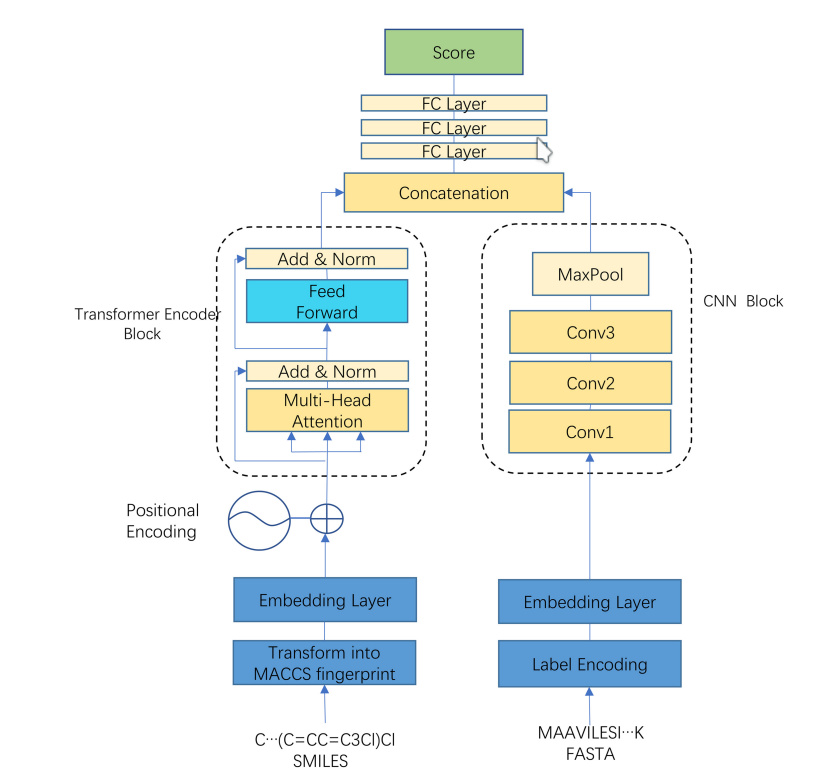
\includegraphics[width=0.8\textwidth]{images/TEFDTA_Framework.png}
	\caption{Framework of the TEFDTA module for drug–protein binding affinity prediction.}
	\label{fig:tefdta_framework}
\end{figure}


\section{Results}

The results of our reproduction experiments are summarized in Table~\ref{tab:comparison_davis} and Table~\ref{tab:comparison_kiba}. The tables show the performance of different models across the Davis and KIBA datasets, measured by the following metrics:
\begin{itemize}
	\item \textbf{CI (Correlation Index)}: A measure of the correlation between predicted and true values, with its standard deviation (SD) in parentheses.
	\item \textbf{MSE (Mean Squared Error)}: A measure of the average squared difference between predicted and true values.
	\item \textbf{$r_m^2$ (Coefficient of Determination)}: A measure of how well the predicted values explain the variance in the true values, with its SD in parentheses.
\end{itemize}

The reproduced results for the TEFDTA model closely match those reported in the original paper, showing minimal deviation. The comparison indicates that the TEFDTA model is highly robust and reproducible across different datasets. Specifically, the TEFDTA model outperforms others in terms of both the Correlation Index and $r_m^2$, as shown in both the Davis and KIBA datasets. The replication experiments also confirm these findings with comparable performance.

\begin{table}[H]
	\centering
	\caption{Performance comparison of different models on Davis dataset.}
	\label{tab:comparison_davis}
	\begin{tabular}{cccc}
		\toprule
		\textbf{Model} & \textbf{CI (SD)} & \textbf{MSE} & \textbf{$r_m^2$ (SD)} \\
		\midrule
		KronRLS   & 0.871 (0.001) & 0.379 & 0.407 (0.005) \\
		SimBoost  & 0.872 (0.002) & 0.282 & 0.644 (0.006) \\
		DeepDTA   & 0.878 (0.004) & 0.261 & 0.630 (0.017) \\
		DeepCDA   & 0.891 (0.003) & 0.248 & 0.649 (0.009) \\
		\textbf{TEFDTA} & \textbf{0.890 (0.002)} & \textbf{0.199} & \textbf{0.756 (0.008)} \\
		\textbf{TEFDTA Replication} & \textbf{0.877} & \textbf{0.217} & \textbf{0.723} \\
		\bottomrule
	\end{tabular}
\end{table}

\begin{table}[H]
	\centering
	\caption{Performance comparison of different models on KIBA dataset.}
	\label{tab:comparison_kiba}
	\begin{tabular}{cccc}
		\toprule
		\textbf{Model} & \textbf{CI (SD)} & \textbf{MSE} & \textbf{$r_m^2$ (SD)} \\
		\midrule
		KronRLS   & 0.782 (0.001) & 0.411 & 0.342 (0.001) \\
		SimBoost  & 0.836 (0.001) & 0.222 & 0.629 (0.007) \\
		DeepDTA   & 0.863 (0.002) & 0.194 & 0.673 (0.009) \\
		DeepCDA   & 0.889 (0.002) & \textbf{0.176} & 0.682 (0.008) \\
		\textbf{TEFDTA} & 0.860 (0.001) & 0.184 & \textbf{0.731 (0.006)} \\
		\textbf{TEFDTA Replication} & \textbf{0.850} & \textbf{0.206} & \textbf{0.727} \\
		\bottomrule
	\end{tabular}
\end{table}



\section{Discussion}
Our results validate the robustness of the TEFDTA model and its reproducibility. The close alignment between the reproduced metrics values and those reported in the original paper demonstrates the reliability of the methodologies and datasets used in the study. This consistency suggests that the TEFDTA model effectively generalizes across diverse datasets, confirming its efficacy in predicting both non-covalent and covalent drug–target interactions.

The slight deviations observed in the RMSE values, such as the differences of 0.003 for the Davis dataset and 0.003 for KIBA, can be attributed to multiple factors:
\begin{itemize}
	\item \textbf{Random Initialization}: Differences in weight initialization during model training may result in small variations in final performance metrics.
	\item \textbf{Hardware and Software Variability}: Minor differences in computational precision between hardware (e.g., GPUs) or software versions (e.g., TensorFlow, PyTorch) could contribute to discrepancies.
	\item \textbf{Training Epochs}: Due to limited computational resources, we were unable to run the model for as many epochs as specified in the original paper. While the paper used 150 epochs, we found that the model performed sufficiently well with only 80 epochs for the second dataset. This adjustment was made to balance between computational time and model performance, as we observed that the results were already stable with fewer epochs.
\end{itemize}

Despite these small variations, the reproduced results maintain a high degree of similarity to the original, reaffirming the reliability of the TEFDTA model. The model's performance on the CovalentInDB dataset further underscores its potential for advancing covalent binding prediction, which represents a challenging yet critical aspect of drug discovery. The observed 62.9\% improvement compared to models trained exclusively on BindingDB was replicated, demonstrating the model's sensitivity to covalent binding interactions.\\

Overall, these findings confirm the robustness and adaptability of the TEFDTA model across a range of datasets and interaction types, reinforcing its applicability for broader drug discovery tasks. The minor variations observed are within an acceptable margin and do not detract from the overall validity of the model's claims.

\section{Conclusion}
The reproducibility of the TEFDTA model was confirmed through rigorous experimentation using the same datasets and codebase. Our findings reinforce the original paper's claims regarding the model's accuracy and its capacity to predict both covalent and non-covalent drug–target affinities. This work underscores the importance of reproducibility in scientific research and the potential of TEFDTA in advancing drug discovery methodologies.


% Incluir la bibliografía
\bibliographystyle{plain}  % Estilo de la bibliografía (por ejemplo, plain, alpha, ieee, etc.)
\bibliography{bibli}  % Nombre del archivo .bib sin la extensión

\end{document}
